\chapter{Energy Estimation} 
\label{chapter-energy-estimation} 

As mentioned earlier, the module EMMA takes the outlyingness of each mode into account. This helps the module determine which modes are important and which are not. The negative log-likelihood (NLL) gives us a measure of outlyingness, having values close to zero for likely data and high values everywhere else. Energy-based models are trained to approximate the NLL but are difficult to train\footnote{See Section\,\ref{sec:ebm}}. This chapter discusses two alternative estimators of NLL obtained training an autoencoder. We will start by explaining the purpose and intuition behind autoencoders. Next, we describe the estimators and how they are derived. And to conclude, a simple experiment is performed to compare the estimators on generated toy data. 

%----------------------------------------------------------------------------------------
%	SECTION 
%----------------------------------------------------------------------------------------

\section{Autoencoder}

Autoencoders (AE) are models trained to reproduce the input to their output. They are composed of two main parts, the encoder $f$ and the decoder $g$. The input $\mathbf{x} \in  \mathbb{R}^L$ is passed through the encoder as $f(\mathbf{x}) = h(W_f\mathbf{x} + \mathbf{b}_f) = \mathbf{u}$ where $h(\cdot)$ is an activation function and $\mathbf{u}$ represents the hidden layer. The decoder is then in charge of reconstructing the input, $g(\mathbf{u}) = W_g\mathbf{x} + \mathbf{b}_g$. The output is often called the reconstruction and is written  $r(\mathbf{x}) = g(f(\mathbf{x}))$. Autoencoders are trained in an unsupervised manner, most of the time using the mean-squared error between input and output as a loss function, $\mathcal{L}_{\text{MSE}} = \lVert r(\mathbf{x}) - \mathbf{x} \rVert_2^2$. But why is it useful to train a model to copy its input? Well to answer this question we need to distinguish two families of autoencoders: the undercomplete and overcomplete autoencoders.

\begin{figure}[!h]
\centering
\begin{subfigure}{.5\textwidth}
\vspace*{4mm}
  \centering
  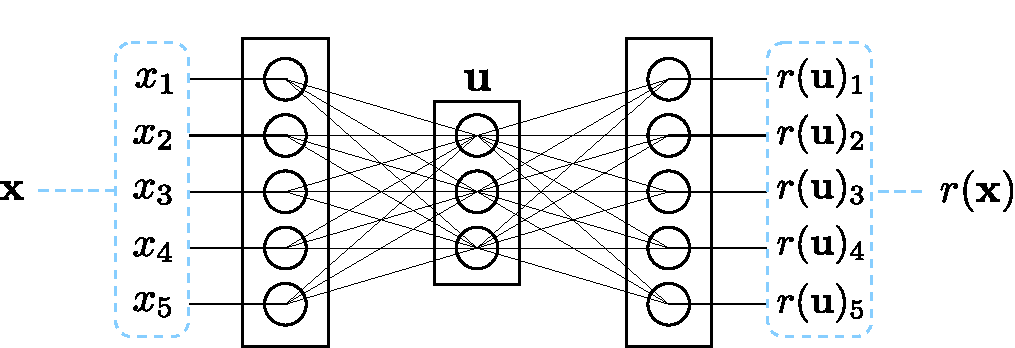
\includegraphics[width=.95\linewidth]{figures/autoencoder-undercomplete}
  \caption{Undercomplete AE}
  \label{fig:undercomplete-ae}
\end{subfigure}%
\begin{subfigure}{.5\textwidth}
  \centering
  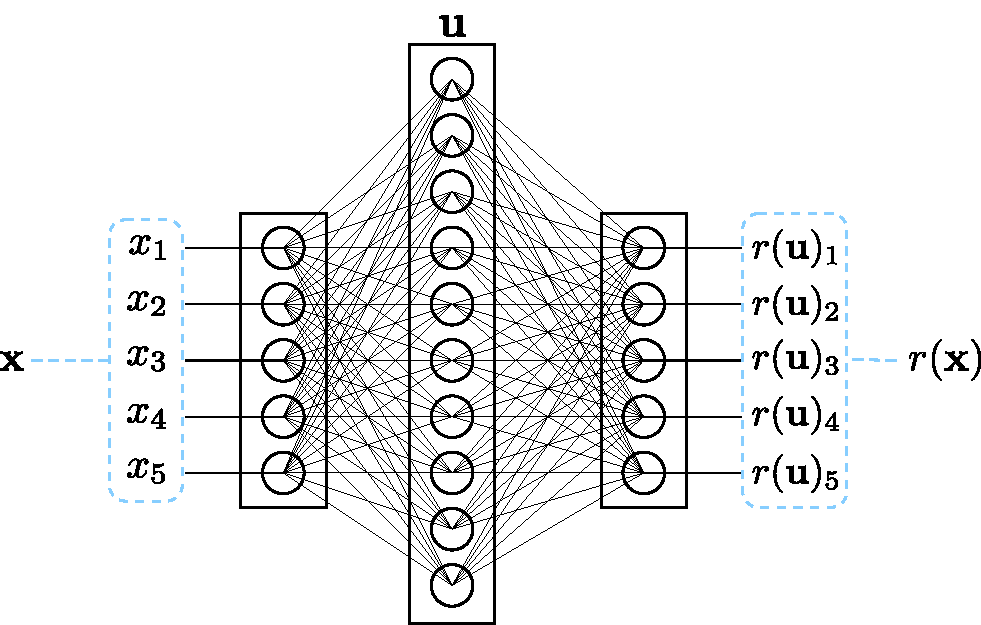
\includegraphics[width=.95\linewidth]{figures/autoencoder-overcomplete}
  \caption{Overcomplete AE}
  \label{fig:overcomplete-ae}
\end{subfigure}
\caption{Two families of autoencoder architectures}
\label{fig:under-over-ae}
\end{figure}

%-----------------------------------
%	SUBSECTION 
%-----------------------------------
\subsection*{Undercomplete}
An autoencoder is undercomplete if the size of the hidden layer $\mathbf{u}$ is smaller than the size of the input/output layers (see Figure \ref{fig:undercomplete-ae}). As a result, the input $\mathbf{x}$ has to pass through a bottleneck, forcing the model to loose some information and keep only the most relevant features. It can be thought of as non-linear principal component analysis \citep{pca-ae-1, pca-ae-2}: the values formed in the hidden layer are a representation in latent space of the input. As can be seen in Figure \ref{fig:reconstruction}, minimizing the mean squared error is similar to minimizing the norm of the vector $r(\mathbf{x}) - \mathbf{x}$.

\begin{figure}[!h]
\centering
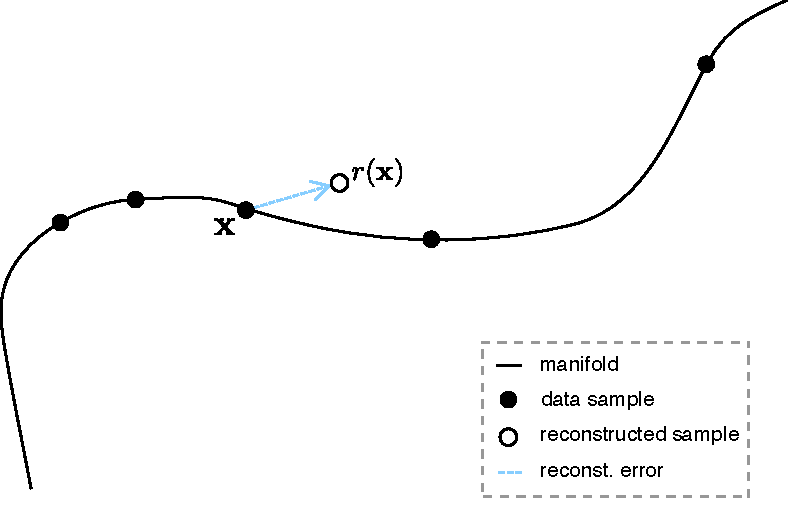
\includegraphics[scale=0.55]{figures/reconstruction}
\caption[Vectorial representation of undercomplete AE]{Vectorial representation of an undercomplete reconstruction process}
\label{fig:reconstruction}
\end{figure}

%-----------------------------------
%	SUBSECTION 
%-----------------------------------
\subsection*{Overcomplete}
Conversely, an overcomplete AE has more hidden units than its input/output layer (see Figure \ref{fig:overcomplete-ae}). Straightforwardly, the model can learn to copy the input to the output through the $L$ hidden units. To spice things up, the input is corrupted before being passed through the encoder. If we force the AE to reconstruct the original input, we now have a model learning to denoise signals. This type of AE is called a denoising autoencoder (DAE). More formally, the input is corrupted with some small isotropic noise $\tilde{\mathbf{x}} = \mathbf{x} + \mathbf{\epsilon}$ with $\epsilon_i \sim \mathcal{N}(0,\,\sigma^{2})$, with the training loss 
\begin{equation}
\mathcal{L}_{\text{MSE}} = \lVert r(\tilde{\mathbf{x}}) - \mathbf{x} \rVert_2^2
\end{equation}
Notice the difference with the loss function of the undercomplete AE. We verify on Figure \ref{fig:reconstruction-dae} that minimizing the loss, $r(\tilde{\mathbf{x}}) \rightarrow \mathbf{x}$, is equivalent to learning to invert the corruption, $r(\tilde{\mathbf{x}}) - \tilde{\mathbf{x}} \rightarrow -(\tilde{\mathbf{x}} - \mathbf{x})$.

\begin{figure}[!h]
\centering
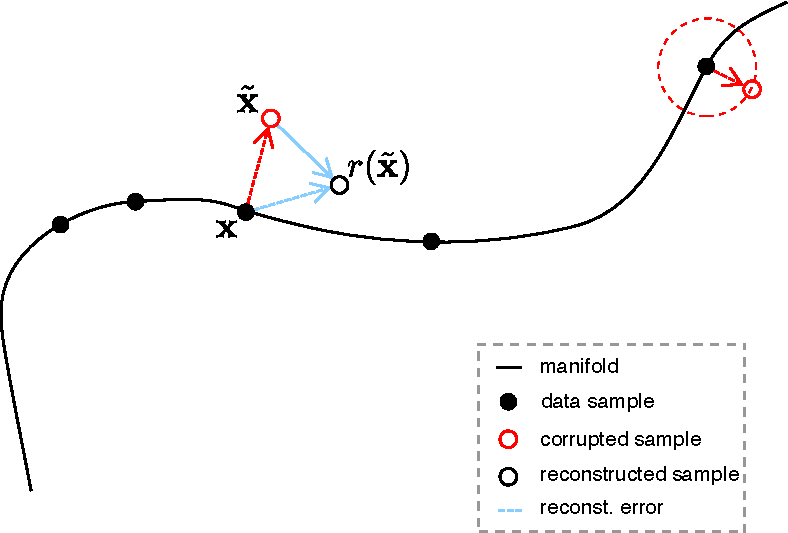
\includegraphics[scale=0.55]{figures/reconstruction-denoising}
\caption[Vectorial representation of overcomplete AE]{Vectorial representation of an overcomplete reconstruction process}
\label{fig:reconstruction-dae}
\end{figure}

%----------------------------------------------------------------------------------------
%	SECTION 
%----------------------------------------------------------------------------------------

\section{Negative log-likelihood Estimators}

The norm of the reconstruction error, $\lVert r(\tilde{\mathbf{x}}) - \tilde{\mathbf{x}} \rVert_2^2$, is sometimes used in the Machine Learning community as a way to detect oultiers. The motivation is that samples far away of the data manifold will have larger reconstruction error than samples close to the manifold. However, as we will see later on in the experiments, the reconstruction error is not a good estimator of the NLL and can lead to false positives.

The authors in \citep{alainbengio} proved that the reconstruction error of a trained denoising autoencoder is proportional to the score (gradient of log-likelihood)
\begin{equation}
r(\tilde{\mathbf{x}}) - \tilde{\mathbf{x}} \propto \frac{\partial \log p(\tilde{\mathbf{x}})}{\partial \tilde{\mathbf{x}}} 
\label{eq:score-reconstruction}
\end{equation} 
To put it differently, the reconstruction error points in the same direction as the corresponding most likely datapoint. To illustrate thisn a DAE is trained on generated circle manifold (more details about the experiment in Section \ref{sec:experiment-I}). As we can see below, the vector field of the reconstruction error does indeed point towards the data manifold.
\begin{figure}[!h]
\centering
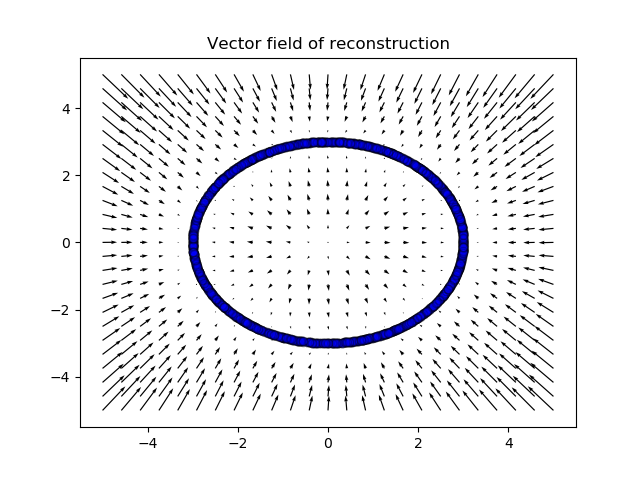
\includegraphics[scale=0.6]{figures/circle-vector-field}
\caption[Vector field circle manifold]{Vector field of reconstruction error on circle manifold. No corruption is applied at test time, the reconstruction error vector is simply the output minus the input.}
\label{fig:vf-circle}
\end{figure}

In \citep{potentialenergy}, authors observed that using tied weights ($W_f = W_g^T$), makes the integrability criterion\footnote{See Section \ref{sec:physics}} satisfied:
\begin{equation}
\begin{split}
\frac{\partial(r(\tilde{\mathbf{x}})_i- x_i)}{\partial x_j} &=  \sum_k W_{ik} \frac{\partial h(W\tilde{\mathbf{x}} + \mathbf{b}_f)}{\partial(W\tilde{\mathbf{x}} + \mathbf{b}_f)}W_{jk} - \delta_{ij}   \\
&= \frac{\partial(r(\tilde{\mathbf{x}})_j- x_j)}{\partial x_i}
\end{split}
\end{equation} 
where $\delta_{ij}$ denotes the Kronecker delta and $W=W_f$. The vector field under those circumstances can be expressed as a gradient of a scalar field $-\Psi$, such that $r(\tilde{\mathbf{x}}) - \tilde{\mathbf{x}} = -\partial \Psi(\tilde{\mathbf{x}})/\partial \tilde{\mathbf{x}}$. In analogy to physics, we can interpret the vector field as a force applied on the input and the scalar field as a potential energy. Thereupon, the reconstruction process can be seen as a gradient descent in the potential energy landscape \citep{potentialenergy}. For our purpose, an important observation to make is that the potential energy is proportional to the NLL,
\begin{equation}
-\frac{\partial \Psi(\tilde{\mathbf{x}})}{\partial \tilde{\mathbf{x}}} \propto -\frac{\partial \log p(\tilde{\mathbf{x}})}{\partial \tilde{\mathbf{x}}} \Rightarrow  \Psi \propto -\log p
\end{equation}
The potential energy being the gradient of the reconstruction error, we can compute $\Psi$ as
\begin{equation}
 \Psi(\tilde{\mathbf{x}}) = -\int (r(\tilde{\mathbf{x}}) - \tilde{\mathbf{x}})d\tilde{\mathbf{x}} 
 \label{eq:psi-int}
\end{equation}
Substituting $f = h(W\mathbf{x} + \mathbf{b}_f)$ and $g = W^T\mathbf{x} + \mathbf{b}_g$
\begin{equation}
\Psi(\tilde{\mathbf{x}})= -\int f(\tilde{\mathbf{x}})d\tilde{\mathbf{x}} - \frac{1}{2} \lVert \tilde{\mathbf{x}} + \textbf{b}_r \rVert_2^2 + \text{const}
\end{equation} 
The intermediate steps between (\ref{eq:psi-int}) and (\ref{eq:potential-prop}) are detailed in \citep{potentialenergy}. In this work we will only use the sigmoid activation function, we solve
\newcommand\boxedB[1]{{\setlength\fboxsep{8pt}\boxed{#1}}}
\begin{equation}
\boxedB{\Psi(\tilde{\mathbf{x}}) =  -\sum_k \log(1 + \text{exp}(W_{.k}^T \tilde{\mathbf{x}} + b_k^f)) + \frac{1}{2} \lVert \tilde{\mathbf{x}} - \textbf{b}_g \rVert_2^2 + \cancel{\text{const}} \propto -\log p(\tilde{\mathbf{x}})}
\label{eq:potential-prop}
\end{equation}
where $W_{.k}^T$ is the $k^{\text{th}}$ column of $W^T$, and $b_k^f$ the $k^{\text{th}}$ element of $\textbf{b}_f$. The consequences of neglecting the constant will be discussed in the next chapter. To sum up, we now have two estimators of the negative log-likelihood being derived from a trained denoising autoencoder: the reconstruction error and the potential energy. The latter being more theoretically grounded.


%----------------------------------------------------------------------------------------
%	SECTION 
%----------------------------------------------------------------------------------------

\section{Experiment I}\label{sec:experiment-I}

In this experiment we are going to generate two simple data manifolds. A denoising autoencoder will then be trained on each manifold. From those autoencoders we will compute the estimators and compare them.

\subsection*{Manifolds}
For no particular reason, we decide to generate a set of $N$ samples $\mathbf{x} \in \mathbb{R}^2$ in the form of a wave and a circle. Both manifolds are generated in two steps. First, N samples are randomly selected in an interval $[0, 2\pi]$. The N samples are written $\mathbf{t}$, and are transformed to manifolds as
$$
\text{wave}  \begin{cases}
      \mathbf{x}_1 = \mathbf{t} - \pi \\
      \mathbf{x}_2 = \sin(\mathbf{t})
    \end{cases}  \qquad \text{circle}  \begin{cases}
      \mathbf{x}_1 = 3\sin(\mathbf{t}) \\
      \mathbf{x}_2 = 3\cos(\mathbf{t})
    \end{cases}
$$
The result of this process can be viewed on Figure \ref{fig:generate-manifold}.
\begin{figure}[!h]
\centering
\begin{subfigure}{.5\textwidth}
  \centering
  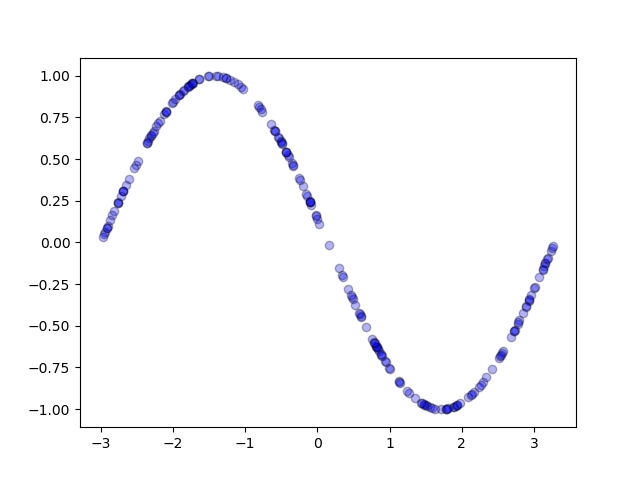
\includegraphics[width=.95\linewidth]{figures/wave-manifold}
  \caption{Wave}
\end{subfigure}%
\begin{subfigure}{.5\textwidth}
  \centering
  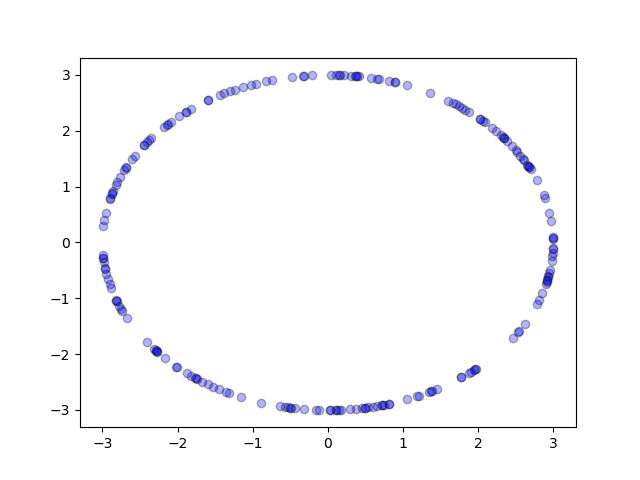
\includegraphics[width=.95\linewidth]{figures/circle-manifold}
  \caption{Circle}
\end{subfigure}
\caption{Manifold generation of 200 samples}
\label{fig:generate-manifold}
\end{figure}

\subsection*{Setup}
Each autoencoder has 8 hidden units and is trained for 25 epochs. The size of the batch is 100, with a corruption noise $\sigma = 0.008$. The used optimizer is \textit{Adam} \citep{kingma} with a learning rate of $1e^{-3}$.

\subsection*{Results}

The autoencoders for both manifolds converged quickly. We observe on Figure \ref{fig:exp1-vector-fields} that the vector fields of the reconstruction error are directed towards the manifolds. We can think of the manifold as sinks in the vector field. Notably, observe the presence of a source in the center of the manifold (see Figure \ref{fig:exp1-vf-circle}).
\begin{figure}[!h]
\centering
\begin{subfigure}{.5\textwidth}
  \centering
  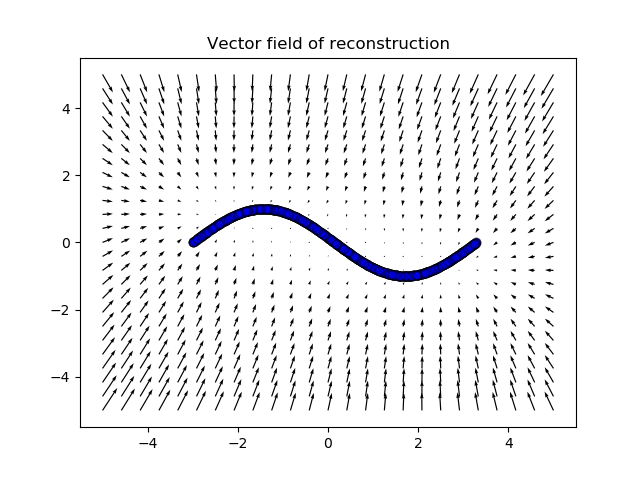
\includegraphics[width=.95\linewidth]{figures/wave-vector-field}
  \caption{Wave}
\end{subfigure}%
\begin{subfigure}{.5\textwidth}
  \centering
  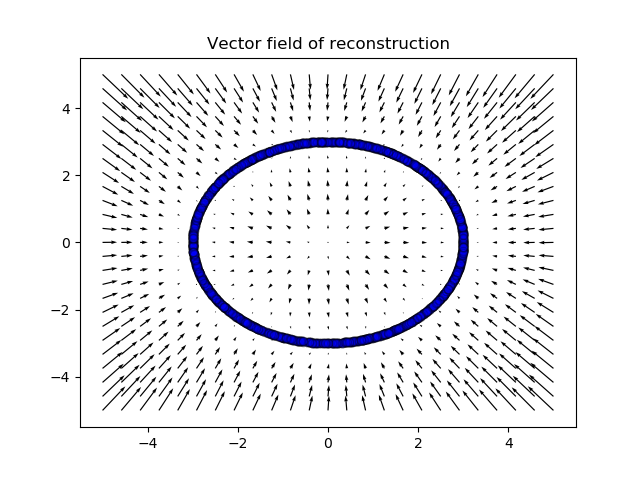
\includegraphics[width=.95\linewidth]{figures/circle-vector-field}
  \caption{Circle}
  \label{fig:exp1-vf-circle}
\end{subfigure}
\caption[Vector fields on wave and circle manifold]{Vector fields of the reconstruction error evaluated on a mesh grid}
\label{fig:exp1-vector-fields}
\end{figure}

Next, the estimators are computed and plotted onto heatmaps (see Figure \ref{fig:exp1-heatmaps}). Not surprisingly, the estimators have low values in the neighbourhood of the manifold and are high everywhere else. More interestingly, a clear difference is observed between the estimators on the circle manifold. This can be explained by the fact that the norm of the reconstruction error at the source is small just as on the manifold itself. A small additional detail is that some potential energies are negative, which is due to the neglected integration constant in Equation (\ref{eq:potential-prop}).
\begin{figure}[!h]
\centering
\begin{subfigure}{.5\textwidth}
  \centering
  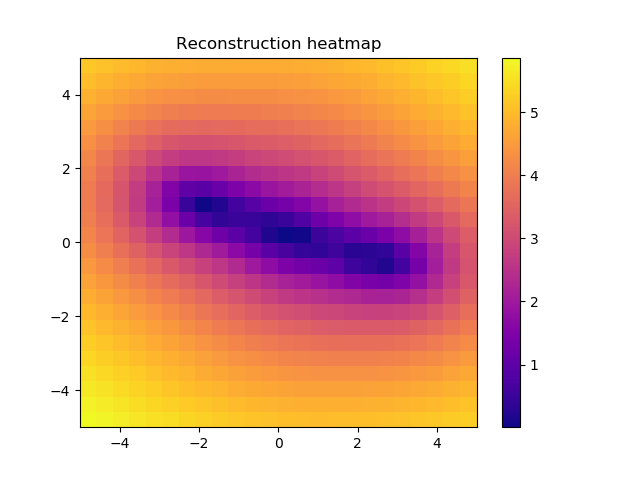
\includegraphics[width=.95\linewidth]{figures/wave-quantifier-reconstruction}
  \caption{Wave - Recontruction}
\end{subfigure}%
\begin{subfigure}{.5\textwidth}
  \centering
  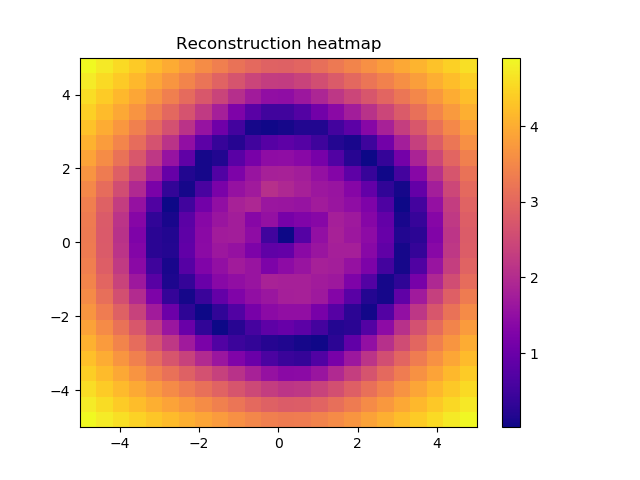
\includegraphics[width=.95\linewidth]{figures/circle-quantifier-reconstruction}
  \caption{Wave - Potential}
\end{subfigure}
\begin{subfigure}{.5\textwidth}
  \centering
  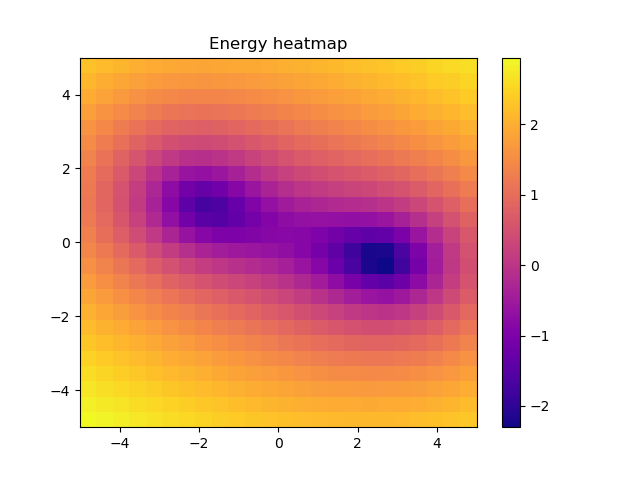
\includegraphics[width=.95\linewidth]{figures/wave-quantifier-energy}
  \caption{Circle - Recontruction}
\end{subfigure}%
\begin{subfigure}{.5\textwidth}
  \centering
  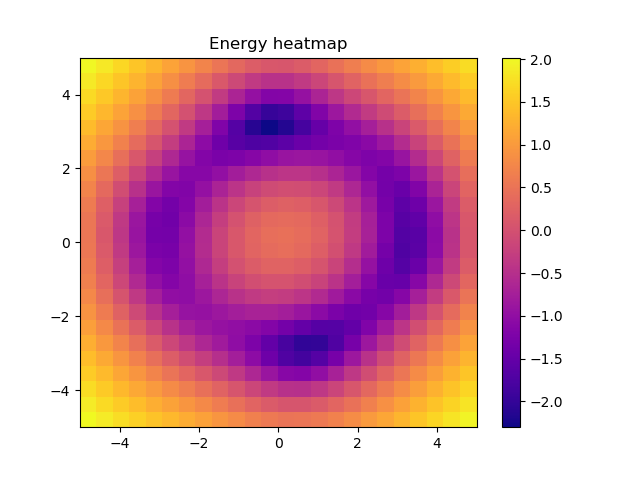
\includegraphics[width=.95\linewidth]{figures/circle-quantifier-energy}
  \caption{Circle - Potential}
\end{subfigure}
\caption[Heatmap of estimators on wave and circle manifold]{Estimators evaluated on wave (left) and circle (right) manifolds}
\label{fig:exp1-heatmaps}
\end{figure}


%----------------------------------------------------------------------------------------
%	SECTION 
%----------------------------------------------------------------------------------------

\section{Limitations}

TODO. The intergrability criterion is guaranteed to be satisfied when using tied weights, this assumption is valid only because there are no more than one hidden layer. Adding more non-linear layers breaks the criterion. Potential energy as it is currently defined cannot directly be applied on convolutional AE, LSTM AE, stacked AE.

Alternative bengio, and others. Future work could investigate if possible to find other potential energy or add constraint on CNN, .. to make it work. Or simply test with current definition and see if it is that bad. 

Scope is to make module that uses any measure of outlyingness. Not to find the best one, somebody else work.